\documentclass[11pt]{article}

\usepackage[utf8]{inputenc}
\usepackage[T1]{fontenc}
\usepackage{lmodern}
\usepackage[margin=1in]{geometry}
\usepackage{amsmath,amssymb}
\usepackage{booktabs}
\usepackage{tabularx}
\usepackage{array}
\usepackage{enumitem}
\usepackage{fvextra}
\usepackage{newunicodechar}
\usepackage{tikz}
\usetikzlibrary{arrows.meta,positioning,fit,backgrounds}
\usepackage[numbers,sort&compress]{natbib}
\usepackage[hidelinks]{hyperref}

\newunicodechar{≠}{\ensuremath{\neq}}
\newunicodechar{∧}{\ensuremath{\wedge}}
\newunicodechar{→}{\ensuremath{\to}}
\newunicodechar{∀}{\ensuremath{\forall}}

\newcommand{\code}[1]{\texttt{#1}}
\newcommand{\lean}[1]{\texttt{#1}}

\title{CogLean: Towards a Cumulative, Machine-Checked Theory of Cognition}
\author{Jeff Shrager}
\date{Draft, November 2026}

\begin{document}
\sloppy
\maketitle

\begin{center}
\fbox{\parbox{0.9\linewidth}{\centering\large\textbf{Draft for Comment}\footnotemark}}
\end{center}
\footnotetext{This draft has \emph{not} been carefully checked by the author. It is likely to contain erroneous citations and details. Think of this as an over-starched blog post. I'm happy to receive constructive feedback at: \texttt{jshrager@gmail.com}}
\medskip

\begin{abstract}
Cognitive architectures such as ACT-R and Soar have long sought to make cognitive theory cumulative, by providing shared computational mechanisms within which models of different tasks can be built and integrated. What such models predict, however, is usually established by running them at chosen parameter settings, and a result established for one model is rarely available, as a result, to another. CogLean pursues a complementary objective: accumulating formally proved theoretical results about cognitive mechanisms. We describe CogLean, a library of cognitive theory in the Lean proof assistant, organized on the model of Mathlib, the community library of formalized mathematics. CogLean is not a new theory of cognition. Its shared library, CogLib, holds representations, mechanisms, theory-neutral statements of phenomena, and machine-checked theorems relating them, and existing theories are expressed as choices of those mechanisms.

CogLean is less about proof, in the usual sense, than about explanation. Its theorems are explanations: deductions of a phenomenon from mechanisms and stated assumptions. They are proved about the same definitions that run as the model, so that when a model changes, any explanation the change invalidates fails to check. We set out the correspondence between scientific notions (model, mechanism, phenomenon, fact, prediction, assumption, explanation) and what they are in Lean, and illustrate it with one phenomenon, confident errors, proved for one memory, for every memory that satisfies three stated laws, and shown to fail for ACT-R's declarative memory. Neither theories nor phenomena need be exact for this to work. Probabilistic mechanisms are handled exactly, as distributions; phenomena can be stated at graded levels of precision. The power law of practice, for example, becomes a family of claims of increasing strength. With these, an average of exponential learners is proved not to be exponential, and ACT-R's base-level learning is proved to produce an exact power law under one practice schedule and, under another, a curve with every qualitative signature of a power law that is nonetheless not one. Companion papers compose theories into a model of multi-digit addition and take the library to concept formation. We distinguish what has been proved from what remains an aspiration.
\end{abstract}

\section{Introduction}
\label{sec:intro}

Making cognitive theory cumulative is an old problem, and much of the work on it has been done by cognitive architectures. Newell's complaint that the field asks nature twenty questions without assembling the answers \citep{newell1973} led to his call for unified theories of cognition \citep{newell1990}. Soar \citep{laird1987,laird2012} and ACT-R \citep{anderson2007} answered it with shared computational mechanisms and constraints: a model of a new task built in the architecture reuses the architecture's theory of memory, learning and control, and models of different tasks can be integrated because they share those commitments. Decades of work by Newell, Anderson, Laird, Rosenbloom and many others have made this the principal means by which cognitive theory accumulates, and the Common Model of Cognition \citep{laird2017} extends it to what several architectures share. CogLean is not the first effort in this direction, and it is not a competitor to, or a replacement for, cognitive architectures.

What architectures accumulate, though, is mainly computational models and the commitments they share. What a model predicts is usually established by running it at chosen parameter settings, and a result established for one model, or one task, is rarely available as a \emph{result} to another: it has to be re-established by running the new model. CogLean pursues a complementary objective. It aims to accumulate formally proved theoretical results about cognitive mechanisms: machine-checked theorems that, once established in one context, can be reused deductively in another, and that can be generalized beyond the commitments of any particular architecture. Nothing prevents an architecture from incorporating such a capability, and its longer-term ambition is to provide a mathematical foundation for reasoning about cognitive architectures themselves. Related arguments that computational modeling forces theories to be made explicit \citep{guest2021}, and that psychology needs explanatory theories, not only tests \citep{vanrooij2021}, motivate the same aim.

The difference has two parts.
\begin{itemize}
  \item \textbf{Accumulating models versus accumulating proved results.} An architecture lets models of different tasks reuse theoretical commitments. CogLean adds the ambition of reusing \emph{theorems} about the mechanisms: a property proved of a memory, say, is available to every model that uses that memory, without re-running anything.
  \item \textbf{Reasoning across architectural commitments.} ACT-R and Soar each embody particular theories of memory, learning and control. CogLean states phenomena and properties of mechanisms independently of any architecture, so that results can be proved for whole classes of mechanisms that satisfy stated laws. The example of Section~\ref{sec:example} is a case: a phenomenon holds for every memory that satisfies three laws, which covers EPAM's discrimination nets but not ACT-R's declarative memory. It also shows the present limits. The laws are proved sufficient, not necessary, and nothing here establishes general equivalence or divergence among architectures.
\end{itemize}

\paragraph{Formalizing explanations.} CogLean's targets are \emph{phenomena}: regularities of behavior, stated without reference to any mechanism. A phenomenon that has been observed is a psychological fact; one that has been derived but not observed is a prediction. CogLean's \emph{explanations} are deductions of a phenomenon from mechanisms and stated assumptions: in Lean, a theorem and the chain of lemmas behind it. This is the deductive-nomological account of explanation \citep{hempel1948}, in which a phenomenon is explained by deducing it from laws and conditions, with the deduction carried through the operation of mechanisms \citep{machamer2000}, and made mechanically checkable. Lean proves conditional propositions: given these mechanisms and assumptions, the phenomenon follows. It does not establish that the assumptions are true of people, or that the phenomenon occurs; that is the business of empirical psychology. What CogLean establishes is the deductive relation between the two. Not every proof explains \citep{steiner1978}, and validity does not rule out the familiar failures of deductive explanation, such as irrelevant premises; which theorems are explanations is a judgment, which CogLean records in the open (Section~\ref{sec:status}). Table~\ref{tab:map} maps these scientific notions onto what they are in Lean. A phenomenon can have several explanations, and a mechanism can take part in explaining several phenomena. A library that accumulates phenomena, mechanisms and explanations can compose them, compare the explanations of one phenomenon, and ask which observations would tell them apart.

\paragraph{Keeping explanations aligned with models.} Cognitive theories are often expressed as programs, and explanations of what the programs do are expressed separately: in prose, in mathematics about an idealization of the program, or in informal reasoning. As models grow and change, the explanations can drift away from what the programs actually do, without anyone noticing. In Lean a definition is both a program and a mathematical object, so the definitions that run as the model are the ones the theorems are about. In the companion paper's model of multi-digit addition \citep{shrager2026multidigit}, for instance, the trial that is executed to produce answers is the same trial the confident-errors theorem reasons about, through its recognition, retrieval and problem solving. When a mechanism changes, every explanation that depends on it is checked again: those the change invalidates fail and must be repaired, and the rest are confirmed. This is perhaps the most important thing Lean contributes. It has limits. Lean keeps explanations aligned with the \emph{formal} model. Whether the formalization is faithful to the original theory (Section~\ref{sec:sim}), whether sampled simulations match the exact distributions (checked statistically), and whether prose such as this paper describes the Lean correctly, remain for people to check.

Mathematics faced a version of the same problem and has made progress on it. Mathlib \citep{mathlib2020}, the community library of formalized mathematics for the Lean proof assistant \citep{demoura2021}, does not propose new mathematics. It provides one shared formal environment, in which definitions are made once, every result is machine-checked, and later work builds on earlier results by citing them. A theorem about groups, once proved, is available to everyone who uses groups. This paper asks whether cognitive theory can be organized the same way, and describes CogLean \citep{coglean}, an initial library built to find out.

The argument rests on four capabilities, in increasing order of importance.
\begin{enumerate}
  \item \textbf{Formalization.} Existing theories are stated as definitions, postulates and theorems. Each theorem's assumptions are explicit.
  \item \textbf{Composition.} Formalized mechanisms are reused in new contexts, and so are the \emph{theorems} about them. A library of reusable cognitive algorithms would be useful software. A library of reusable \emph{results} is a contribution to theory. The companion paper composes EPAM's recognition, Siegler and Shrager's distributions of associations and a problem solver into a model of multi-digit addition, and derives its consequences largely from the components' theorems \citep{shrager2026multidigit}.
  \item \textbf{Generalization over classes.} Phenomena are stated independently of mechanisms, and theorems are proved for every mechanism that satisfies stated laws, and for every representation with stated properties. A new theory that satisfies the laws inherits the results.
  \item \textbf{Discovery}, in a limited sense. Formalization exposes unstated assumptions, results that hold only under conditions, and conditions under which theories diverge. It can also expose an ambiguity in a theory: in Appendix~\ref{app:chris}, an informal claim of the strategy-choice model turns out to follow from its postulates under one assumption about learning and not under another.
\end{enumerate}

\paragraph{The aspiration.} The longer-term objective of CogLean is not merely to provide executable implementations of cognitive theories, or even machine-checked proofs about particular implementations. It is to develop a cumulative mathematical theory of cognition, in which the assumptions responsible for psychological phenomena can be isolated, compared and generalized. Rather than asking only what a particular model predicts at a particular parameter setting, we seek to establish which properties of cognitive mechanisms and representations are sufficient (or, where possible, necessary) for classes of behavioral phenomena. Such results would characterize relationships among theories, identify their common commitments, reveal the conditions under which they diverge, and let new theories inherit established results by satisfying previously formalized laws. This paper does not achieve that. It shows that some of the constituent capabilities already work, and Section~\ref{sec:program} separates what is proved from what is aspiration.

Section~\ref{sec:coglean} describes the library and its vocabulary. Section~\ref{sec:example} works one example. Section~\ref{sec:squishy} takes up theories and phenomena that are not exact, with learning curves as the case. Sections~\ref{sec:kinds}--\ref{sec:sim} sort the kinds of result and say what a proof does and does not show. Section~\ref{sec:discussion} places CogLean among other formal work and cognitive architectures, and lists directions. Appendix~\ref{app:chris} follows a hypothetical modeler through the method, from a phenomenon to a theorem and back from a proposed regularity to the assumptions it requires.

\section{CogLean}
\label{sec:coglean}

\subsection{Organization}

CogLean has four layers (Figure~\ref{fig:arch}).
\begin{itemize}
  \item \textbf{Lean}, the formal language and proof checker. CogLean uses only Lean's core, not Mathlib, and every probability is an exact rational number.
  \item \textbf{CogLib}, the general library. It holds:
  \begin{itemize}
    \item representations: feature codes, finite probability distributions, semantic networks, frames;
    \item memory structures: discrimination nets, an ACT-R-style activation memory;
    \item processes: discrimination learning, sampled retrieval with a confidence criterion, ``recognize, then retrieve, else back up'', spreading activation, and a decision cycle with impasses and repairs;
    \item an interface any memory can implement (a \emph{retriever}: study an item, retrieve a distribution over stored items);
    \item theory-neutral statements of phenomena and laws, such as the serial-position effect, the shape of a learning curve, or the law that retrieval of a studied item is certain.
  \end{itemize}
  CogLib imports no theory.
  \item \textbf{Theories}, each a package that states its postulates as choices of CogLib constructs, cited to their sources, and proves its phenomena.
  \item \textbf{Applications}, models of particular tasks assembled from theories and library mechanisms, with the task's own knowledge.
\end{itemize}

\begin{figure}[t]
\centering
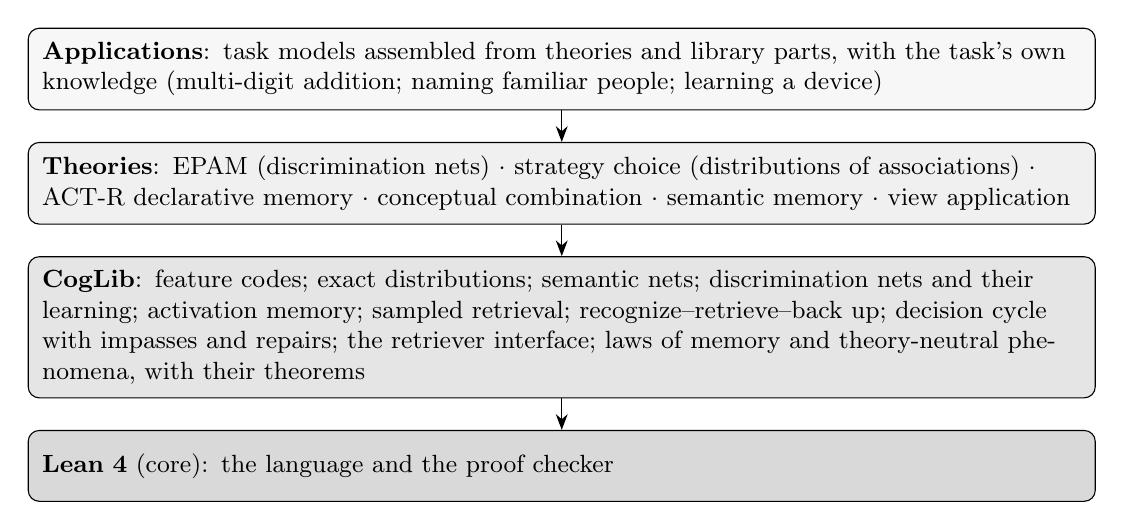
\begin{tikzpicture}[font=\small,
  layer/.style={draw, rounded corners, minimum height=9mm, text width=13.2cm, align=left, inner sep=5pt},
  arr/.style={-{Stealth[length=2mm]}}]
  \node[layer, fill=black!3] (app) {\textbf{Applications}: task models assembled from theories and library parts, with the task's own knowledge (multi-digit addition; naming familiar people; learning a device)};
  \node[layer, fill=black!6, below=4mm of app] (th) {\textbf{Theories}: EPAM (discrimination nets) $\cdot$ strategy choice (distributions of associations) $\cdot$ ACT-R declarative memory $\cdot$ conceptual combination $\cdot$ semantic memory $\cdot$ view application};
  \node[layer, fill=black!10, below=4mm of th] (lib) {\textbf{CogLib}: feature codes; exact distributions; semantic nets; discrimination nets and their learning; activation memory; sampled retrieval; recognize--retrieve--back up; decision cycle with impasses and repairs; the retriever interface; laws of memory and theory-neutral phenomena, with their theorems};
  \node[layer, fill=black!15, below=4mm of lib] (lean) {\textbf{Lean 4} (core): the language and the proof checker};
  \draw[arr] (app) -- (th); \draw[arr] (th) -- (lib); \draw[arr] (lib) -- (lean);
\end{tikzpicture}
\caption{The layers of CogLean. Arrows point from a layer to what it imports. Each layer's theorems are available to the layers above it.}
\label{fig:arch}
\end{figure}

The contribution is not a programming language or a new syntax for cognitive models. Any model could be written in Lean as a program. What CogLean contributes is an \emph{organization} of theoretical knowledge: mechanisms defined once, phenomena stated independently of any mechanism, and theorems relating them, all in one place where later work can cite them. CogLean is far from Mathlib's scale or maturity. It is a demonstration that the approach can work, not a finished library.

\subsection{Mechanisms, representations, phenomena, theorems and conditions}
\label{sec:kindsobj}

A cognitive model combines kinds of commitment that conventional implementations tend to intertwine. CogLean keeps them apart.
\begin{enumerate}
  \item \textbf{Mechanisms and their postulates}: definitions, such as how a discrimination net sorts a code, or how retrieval samples an answer in proportion to its associative strength.
  \item \textbf{Representations}: which features encode a stimulus, and what information those features preserve. A representation is a parameter of the mechanisms, and its properties can be stated separately (``every digit has a feature saying whether it is zero'').
  \item \textbf{Phenomena}: predicates over a task's outcomes (for example, distributions of answers and of the strategy route that produced them, or a learning curve), stated without reference to any mechanism. A predicate asserts nothing. It is a target, which some mechanism may or may not be proved to satisfy.
  \item \textbf{Theorems}: proofs that a mechanism, or every mechanism of a class, produces behavior satisfying a predicate.
  \item \textbf{Conditions}: the hypotheses under which a theorem holds. Some are situational (``stimulus $x$ is confused with $q$''), some are empirical premises that remain unexplained (``$q$'s associations are sharp''), and some are well-formedness requirements (``the strengths have positive total'').
\end{enumerate}
A theorem that has a phenomenon among its hypotheses is a relation between phenomena, not a prediction of a model. It becomes a prediction only when some mechanism discharges the hypothesis by proving it. CogLean's catalog of theorems, generated from Lean, marks such conditional results mechanically \citep{coglean}.

Table~\ref{tab:map} maps these kinds onto the scientific notions of the introduction. The assumptions of an explanation are postulates, conditions and laws. None is a Lean \code{axiom}: a law of memory is a hypothesis in the way the group axioms are hypotheses in Mathlib, fields that anything claiming to be a group must supply.

\begin{table}[t]
\centering\small
\begin{tabularx}{\linewidth}{@{}>{\raggedright\arraybackslash}p{0.3\linewidth}>{\raggedright\arraybackslash}X@{}}
\toprule
Scientific notion & In CogLean and Lean \\
\midrule
Model (the program) & executable definitions: the same ones that are run, exactly or by sampling \\
Mechanism (postulate) & a CogLib process, chosen by a theory and cited to its source \\
Representation & a parameter (an encoding), with its properties stated as propositions \\
Phenomenon & a predicate over a task's outcomes, stated without any mechanism: a target \\
Psychological fact & a phenomenon judged to hold of people: outside Lean \\
Prediction & a theorem's conclusion about a phenomenon not yet observed \\
Assumption: condition & a hypothesis of a theorem \\
Assumption: law & a proposition about a mechanism, proved for a family or required by a class theorem \\
Explanation & a theorem and its chain of lemmas: mechanisms and assumptions entail the phenomenon \\
Deduction & what Lean's kernel checks \\
Illustration, witness & a computed value at one setting (\code{decide}, \code{\#eval}): not an explanation \\
Lean's own axioms & \code{propext}, \code{Quot.sound}, \code{Classical.choice}: logic, not scientific assumptions \\
\bottomrule
\end{tabularx}
\caption{Scientific notions and what they are in CogLean.}
\label{tab:map}
\end{table}

Shared definitions make theories comparable at the level of proofs. For example, CogLib proves once that any learner whose learning never disturbs what it already knows reaches a learning criterion (\lean{criterion\_of\_nonInterference}). It separately proves that discrimination-net learning never disturbs prior learning (\lean{netLearner\_nonInterference}). EPAM's learning to criterion then follows in a line, and so will that of any later theory whose learning is non-interfering.

\section{An example: confident errors}
\label{sec:example}

One phenomenon, followed from its statement to its explanations, shows the parts working together. The task is as simple as possible: naming familiar people. A face is a code, a vector of features. Memory recognizes it as a familiar face, or as nothing. The recognized person's name associations are then searched, as in the distributions-of-associations (DOA) model of strategy choice \citep{siegler1984}: a name is sampled in proportion to its strength and stated if its strength exceeds a criterion, for up to $n$ searches. If nothing is recognized, or no name clears the criterion, the person falls back on a backup, here ``don't know''. That is CogLib's \code{recognizeRetrieve}, a composition of recognition, retrieval and backup for any task (\code{CogLib/Process/RecognizeRetrieve.lean}); the companion paper uses the same composition for multi-digit arithmetic, with a problem solver as the backup \citep{shrager2026multidigit}.

\paragraph{The phenomenon.} A familiar error is to greet a stranger confidently by the wrong name. CogLib states the pattern once, as a predicate over distributions of answers and the route that produced them (\code{CogLib/Phenomena/ConfusionErrors.lean}):
\begin{Verbatim}[fontsize=\small]
def ConfusionErrorPattern trial wholeWrong isWhole isBackup x q : Prop :=
  prob (trial q) (wholeWrong q) = 0 ∧                            -- (i)
  prob (trial x) (wholeWrong x) = prob (trial x) isWhole ∧       -- (ii)
  prob (trial x) isBackup = prob (trial q) isBackup              -- (iii)
\end{Verbatim}
For any stimuli and outcomes: (i) the familiar $q$ is never answered wrongly from memory; (ii) every answer to $x$ from memory is wrong; (iii) $x$ uses the backup exactly as often as $q$. The definition names no mechanism. Mechanism-independent is not the same as directly observable, however: (ii) and (iii) refer to the route that produced an answer, which an answer alone does not reveal; applying the predicate to people requires measuring the route, for instance by latency or report. Equal backup use is also not low backup use, so CogLib states a stronger phenomenon too, \lean{ConfidentErrors r}: the pattern with backup use at most $r$.

\paragraph{An explanation from mechanisms.} \lean{RR.confident\_errors} proves the pattern for \code{recognizeRetrieve}, for any task, encoding, strengths, criterion, search length and backup, under these conditions:
\begin{itemize}
  \item $q$ is recognized as itself, and $x$ is recognized as $q$, for certain;
  \item $q$'s associations are \emph{sharp}: only its correct answer clears the criterion;
  \item the correct answers differ, and the distributions involved are proper.
\end{itemize}
The proof combines three lemmas: an item recognized as a sharp $q$ gets only $q$'s answer; so all of $x$'s retrieved answers are wrong; and backup use after certain recognition as $q$ depends only on $q$'s associations. No hypothesis mentions errors, or any relation between errors and backup use.

\paragraph{An instance, and a witness.} EPAM \citep{feigenbaum1959,feigenbaum1962} recognizes a code by sorting it down a discrimination net of feature tests. Let EPAM learn two faces, Ann's and Bob's, that differ in their first feature, and let a stranger, Carl, share Bob's first feature. The net tests only that feature, so it recognizes Carl as Bob. With each face's own name at strength $.90$, others at $.01$, and criterion $.50$, the conditions hold, and confident misnaming follows for every search length (\lean{Exp.FaceNaming.epam\_confident\_misnaming}, \code{Experiments/FaceNaming.lean}). At search length 1, Carl is called Bob with probability $45/46$, and says ``don't know'' with probability $1/46$, exactly as often as Bob does (\lean{epam\_values}). The numbers are a witness: they show the conditions can be met, not why the pattern holds.

\paragraph{An explanation for a class of memories.} The first condition is about one net. \lean{RR.confident\_errors\_of\_laws} replaces it with three laws, stated theory-neutrally against the retriever interface (\code{CogLib/Phenomena/RetrievalLaws.lean}):
\begin{itemize}
  \item \emph{determinacy}: retrieval calls up a single item for certain;
  \item \emph{certainty}: a studied item retrieves itself;
  \item \emph{stability}: studying one item does not change another's retrieval of itself.
\end{itemize}
Any memory with the three laws exhibits the pattern, given only that the stranger can be taken for a studied item, sharp associations, and different correct answers. A new theory of memory inherits the result by proving the laws, without reproving anything about recognition, retrieval or backup. CogLean's theory matrix (\code{CogMatrix/}) proves, for each memory family and law, whether the family has the law at every setting, never has it, or lacks it at some setting. EPAM's net has all three. ACT-R's declarative memory \citep{anderson2007}, with base-level activation, partial matching and a retrieval threshold, has none, at any setting. The face-naming result follows again, from EPAM's laws (\lean{epam\_confident\_misnaming\_of\_laws}).

\paragraph{What failing the laws does and does not show.} That the class theorem does not cover ACT-R does not show that ACT-R cannot produce similar errors. In the same task with ACT-R's memory, Carl is called Bob with probability $225/391$, but can also be called Ann, and says ``don't know'' more often than Bob does, so part (iii) fails (\lean{act\_more\_dont\_know}). That is a counterexample at one setting. The library also proves a graded version, which needs no certainty: if $x$ calls up $q$, and $q$ calls up itself, each with probability at least $1-\delta$, the pattern holds to within $2\delta$ (\lean{RR.confident\_errors\_graded}). ACT-R's memory meets that condition when the context primes $q$ strongly enough, and for every $\delta>0$ some degree of priming suffices (\lean{RR.act\_priming\_confident\_errors}). So confident errors have at least two explanations in the library, from discrimination and from partial matching with priming, and they differ in an observation: EPAM's errors follow the features a stranger shares with a stored face, while primed ACT-R's follow the context, such as who was just seen. That is the shape of result a cumulative library should produce. One phenomenon, several explanations, each with its assumptions explicit, and the observations that would tell them apart.

\section{When theories and phenomena are not exact}
\label{sec:squishy}

Deduction might seem to need exact theories and exact phenomena. Neither is required. What has to be explicit is the relation asserted between them.

\paragraph{Mechanisms.} Three cases should be kept apart.
\begin{enumerate}
  \item \textbf{A probabilistic mechanism.} A mechanism that makes random choices, with known probabilities, is still precise. DOA samples an answer in proportion to its strength; the distribution of outcomes is a mathematical object, and CogLib computes and reasons about it exactly, as a finite distribution, composed through every later step without sampling. Everything in Section~\ref{sec:example} is of this kind.
  \item \textbf{Monte Carlo.} When the exact distribution is defined but expensive to compute, it can be estimated by running the mechanism many times. That does not make the theory imprecise, only its consequences harder to calculate. CogLean's simulations run the library's own definitions, with seeded sampling, and are checked against the exact distributions where both are available. Such results are statistical estimates, and should be reported as such, alongside the deductive ones.
  \item \textbf{An incompletely specified mechanism.} When part of a model is a heuristic, a lookup table or a process whose distribution is unknown, deduction can still proceed, but only with that part as a parameter and its required properties as conditions. The sharp associations of Section~\ref{sec:example} are such a premise: an empirical assumption the library does not yet derive.
\end{enumerate}

\paragraph{Phenomena.} A regularity can be characterized at several levels of precision, and a mechanism may yield some and not others. Take the power law of practice \citep{newell1981}, which says that the time $T(n)$ to perform a task after $n$ trials falls as $a n^{-b}$. CogLib states the claims it bundles separately, as predicates on a curve over a range of trials (\code{CogLib/Phenomena/LearningCurve.lean}):
\begin{itemize}
  \item \emph{improvement}: performance never gets worse;
  \item \emph{diminishing returns}: each trial's gain is no larger than the last;
  \item \emph{diminishing relative returns}: each trial's proportional gain is smaller than the last;
  \item \emph{approximately a power law}: within a relative tolerance $\varepsilon$ of scale invariance, $T(kn) = r\,T(n)$;
  \item \emph{an exact power law}: scale invariance itself, with $r = k^{-b}$;
  \item and, for comparison, \emph{exponential}: $T(n+1) = s\,T(n)$.
\end{itemize}
Scale invariance is how a power law is stated with exact rationals, since $n^{-b}$ is generally irrational. The predicates are mathematical. Whether noisy data ``look like'' a power law, which might mean that a power function fits well, or fits better than an exponential, or merely that gains diminish, is a different, statistical proposition, and a deduction does not settle it.

Some relations among these follow without any mechanism. A power curve has diminishing relative returns; an exponential curve does not, because its proportional gain is constant; and no positive curve is both exponential and scale-invariant over a range (\lean{shiftRatio\_not\_scaleRatio}). So the two are different phenomena, not two descriptions of one. More interesting is a result about aggregation. The average of two exponential learners with different rates has strictly diminishing relative returns, a signature of a power curve, and so is not exponential, although each learner is exactly exponential (\lean{mix\_not\_shiftRatio}). This is the old warning that group curves need not have the form of individual ones \citep{estes1956}, which reappears in the debate over whether individual practice curves are power or exponential \citep{heathcote2000}, here as a theorem.

\paragraph{A mechanism, and two practice schedules.} ACT-R's base-level learning adds a decaying trace for each use of a chunk, and retrieval time falls as activation rises \citep{anderson2007}. With decay 1, the case in which every quantity stays rational, CogLib proves the shape of the resulting practice curves (\code{CogLib/Process/Practice.lean}):
\begin{itemize}
  \item \textbf{Massed practice, tested after a delay}: latency is exactly $FL/n$, a power law with exponent 1 (\lean{Act.massed\_scaleRatio}).
  \item \textbf{Spaced practice, tested after each trial}: latency improves, with diminishing returns and diminishing relative returns (\lean{Act.spaced\_improves}, \lean{spaced\_diminishing}, \lean{spaced\_diminishingRelative}), every qualitative signature of a power law. Yet no power law fits it over long ranges: for any ratio below 1, doubling practice eventually shrinks latency by less (\lean{Act.spaced\_not\_powerLaw}). The curve is logarithmic. Over trials 1 to 8 it is nonetheless within 7.5\% of a power law with exponent about $0.47$ (\lean{spaced\_looks\_like\_powerLaw}, a witness).
\end{itemize}
Three points follow. Whether this mechanism ``produces the power law of practice'' depends on the schedule, a condition, not on the mechanism alone. A curve can have every qualitative signature of a power law over an experimentally typical range without being one. And several different mechanisms, here spaced base-level learning and averaged exponential learners, produce the same power-like signatures, so the signatures alone do not identify a mechanism. ACT-R's usual decay, 0.5, needs real powers, so it is treated in a separate package that uses Mathlib's real analysis (\code{ACTR/}), outside the core library. There, the rational predicates are proved to agree with their real-valued forms (\lean{ACTR.scaleRatio\_iff\_cast}; scale invariance at doubling is a power law with exponent $-\log_2 r$, \lean{powerLaw\_of\_scaleRatio}), and for every decay $0 \le d < 1$, spaced practice is proved to be approximately a power law with exponent $1-d$: for any tolerance, beyond some trial (\lean{ACTR.spacedR\_approx\_powerLaw}). The proof squeezes the sum of decaying traces between two integrals. This is Anderson's account of the power law of practice, made checkable. So in ACT-R, whether there is a power law, and its exponent, depend on the decay as well as the schedule.

CogLean does not require psychological theories or phenomena to be exact. It requires the relations asserted between them to be explicit enough to reason about.

\section{Kinds of results}
\label{sec:kinds}

Table~\ref{tab:kinds} sorts results by what they rest on. A reader should be able to tell which statements are library facts about mechanisms, which are deductions from a composition, which hold only given further conditions, which hold for whole classes of mechanisms, which relate phenomena to each other, and which are values at chosen settings. Not every theorem is a psychological prediction, and none here is an empirical finding: the conditional, compositional and class-level results become empirical predictions about people only once their conditions can be identified in people and the predictions tested.

\begin{table}[t]
\centering
\small
\begin{tabularx}{\linewidth}{@{}p{0.21\linewidth}Xp{0.26\linewidth}@{}}
\toprule
Kind & Examples & What they rest on \\
\midrule
\textbf{Library facts}: properties of mechanisms, needed for reuse & a sample from positive strengths is a probability distribution; two evaluators of a trial give the same distribution; two-stage draws regroup & the definitions, and well-formedness \\
\addlinespace
\textbf{Compositional deductions}: hold at every setting of the composed mechanisms & after certain recognition as $q$, backup use is that of $q$'s associations alone, whatever is recognized & the composed mechanisms \\
\addlinespace
\textbf{Conditional}: hold given stated conditions & confident errors; ACT-R's practice curves, given a schedule & recognition conditions; sharp associations (an unexplained empirical premise); the schedule \\
\addlinespace
\textbf{Class-level}: hold for every mechanism satisfying stated laws & confident errors for any memory with three laws; learning to criterion for any non-interfering learner; which families have the laws & the laws, which are not claimed to describe people \\
\addlinespace
\textbf{Relations between phenomena} & power and exponential curves are distinct; an average of exponentials is not exponential & the predicates alone \\
\addlinespace
\textbf{At chosen settings}: exact values & face-naming probabilities under EPAM and ACT-R; a spaced curve within 7.5\% of a power law over trials 1--8; counterexamples at a setting & a chosen encoding, history, strengths and parameters \\
\bottomrule
\end{tabularx}
\caption{Results, by kind.}
\label{tab:kinds}
\end{table}

\paragraph{The role of numerical examples.} Values computed at a chosen setting do five things. They show that independently formalized mechanisms compose into a model that runs; that a theorem's hypotheses can actually be met; that model families make different predictions, as constructive witnesses; that the abstract results can be understood through cases; and that the formal model can be checked against an independent implementation (Section~\ref{sec:sim}). They are illustrative. They depend on chosen encodings, learning histories, strengths, criteria and parameters, they are not fitted to data, and a simulation could produce comparable numbers. A value computed by \code{decide} at one setting is a witness, not an explanation: it shows that something happens there, not why. The explanation is the theorem that covers every setting meeting its conditions.

\section{The scientific status of proofs}
\label{sec:status}

\paragraph{Validity is not empirical adequacy.} A proof establishes that a conclusion follows from its premises. It does not establish that the premises are true of people. Confident misnaming follows from CogLean's formalization of EPAM and DOA. Whether people make such errors, and whether they make them for this reason, are empirical questions.

\paragraph{Validity is not explanation either.} For a theorem to be an explanation, its premises must characterize mechanisms independently, and not restate the phenomenon. An earlier version of CogLib's serial-position result illustrates the difference. Its mechanism was a schedule on which item $i$ was learned on trial twice its distance from the nearer end. Proving that this produces a bowed error curve was valid, but the bow was in the definition. The current version derives the order of learning from a rule over any set of anchors: items nearer an anchor are attended first. The same rule then has a second consequence, the isolation (von Restorff) effect, when a distinctive item serves as an anchor (\code{CogLib/Control/Serial.lean}). The result is still close to its premises. But one mechanism now answers to two phenomena, which is a real test.

The repository records an explicit audit of this kind for its headline results (\code{notes/EXPLANATORY\_AUDIT.md}). It sorts each result by how far it lies from its premises:
\begin{itemize}
  \item \emph{definitional}: a restatement of the definitions;
  \item \emph{close}: the pattern is largely in the mechanism;
  \item \emph{derived}: it follows from premises that do not mention it;
  \item \emph{compositional}: it needs two or more mechanisms working together.
\end{itemize}
Not every CogLean theorem is a psychological explanation. Some are properties of algorithms, needed library facts that explain nothing on their own; some are relations between laws or between phenomena; some, such as confident errors, are compositional. Making these distinctions visible is part of the method: Lean shows every premise, and the judgment of what the premises contain is written down, in the open.

\section{Checking the formalization}
\label{sec:sim}

Lean guarantees that the theorems follow from the definitions. It does not guarantee that the definitions say what the prose model says. The companion paper tests that link for the multi-digit model with an independent implementation that could not simply copy the first \citep[cf.\ N-version programming,][]{avizienis1985}. The model was written as a prose specification, with no Lean names, theorems or predictions. Checks were committed before any simulator existed, each naming a theorem, the observable statistic and a tolerance. A fresh AI agent, given only the specification, wrote the simulator. Every check whose hypothesis arose passed, and hundreds of outcome frequencies matched Lean's exact distributions. The simulation also found what the proofs did not: hypotheses that never arose in the states learning produced, a gap at zero strength, and an unstated assumption that decides a predicted learning sequence \citep{shrager2026multidigit}.

Three standards are involved, and they should not be confused: logical correctness, which Lean checks; behavior in the states that learning actually produces, which simulation can probe; and empirical adequacy, which only data about people address.

\section{Discussion}
\label{sec:discussion}

\subsection{Relation to previous formal work}

CogLean is not the first formalization or mechanical verification of a cognitive theory. Formal specification of cognitive architectures goes back at least to a specification of Soar in Z \citep{milnes1992}. It covered the architecture completely but at a low level, and it could not be executed. Cooper, Fox, Farringdon and Shallice argued that better theories would come from languages designed for specifying cognitive models, and gave one, Sceptic, an executable specification language in which they implemented several models, including Soar \citep{cooper1996}. Stewart and West rebuilt ACT-R in order to separate its core commitments from implementation detail and to explore alternative components \citep{stewart2007}. That anticipates CogLean's interest in interchangeable mechanisms, in an executable setting. Ragni and colleagues proposed a formal framework into which architectures such as ACT-R and Soar can be embedded for comparison \citep{ragni2018}.

For ACT-R in particular, Gall and Frühwirth gave an abstract operational semantics, a translation to Constraint Handling Rules proved sound and complete with respect to it, and a decidable confluence test \citep{gall2018,gall2017confluence}. Langenfeld, Westphal and Podelski translated ACT-R models to timed automata for exhaustive defect analysis \citep{langenfeld2019}, and proved their timed-automaton semantics correct at the level of architectural components \citep{langenfeld2021}. Macklem and Mili proposed specification languages and algorithms for checking cognitive models against requirements \citep{macklem2006}. In the context of the Common Model of Cognition \citep{laird2017}, Ganeriwala and colleagues have proposed enabling formal verification of cognitive models \citep{ganeriwala2025}. They have also compiled Soar models to discrete-time Markov chains for probabilistic model checking in PRISM \citep{ganeriwala2026,kwiatkowska2011}, which addresses stochastic behavior, as CogLean's exact distributions do. Outside architectures, verbal theories have been formalized as logic programs \citep{rohner2021} and as communicating automata \citep{finkel2025}. Fisher and colleagues derived critical tests of ACT-R from its core architectural assumptions, as theorems over a space of model classes \citep{fisher2025}, an aim close to CogLean's separation of what follows from a theory's core.

\paragraph{Model verification and theoretical deduction.} Three approaches to establishing what a cognitive model does should be kept apart.
\begin{itemize}
  \item \textbf{Simulation} samples executions to estimate behavioral outcomes.
  \item \textbf{Probabilistic model checking}, as in PRISM, analyzes a specified state-transition model exhaustively, often by numerical methods, to establish properties or compute probabilities over its whole state space. This is formal verification, not simulation. It can also treat parameters symbolically, giving a property or probability as a function of them \citep{hahn2011}.
  \item \textbf{Deductive theorem proving}, as in CogLean, establishes results for whole classes of models that satisfy stated theoretical assumptions. They are independent of particular parameter settings and of any finite enumeration of states.
\end{itemize}
The important distinction is therefore not between simulation and formal verification, but between \emph{model verification} and \emph{theoretical deduction}. Model checking primarily verifies properties of a particular formalized system, or of a parameterized family of them. CogLean's principal objects are the theories themselves: reusable representations, mechanisms, assumptions and theorems. Its aim is to establish general consequences of those theories, and to derive further results by composing independently formalized mechanisms. The approaches are complementary, not competitors. A model checker can verify a large, detailed model that would be laborious to reason about deductively. A theorem can state what every such model must do, and why.

CogLean does not introduce formal methods to cognitive science. What is distinctive, relative to this work, is a combination of emphases, few of them entirely new on their own:
\begin{itemize}
  \item \textbf{Theorems over classes of models}, not properties of one model or one parameterized family. CogLean's theorems quantify over every encoding, net, strength set and backup, and, through laws, over every memory.
  \item \textbf{Phenomena and laws stated theory-neutrally}, so that rival mechanisms can be tested against the same statement.
  \item \textbf{Reusable proofs across independently developed theories.} The previous work formalizes one architecture or model at a time. CogLean's companion paper composes theorems proved separately for EPAM, DOA and a problem solver into results about their combination.
  \item \textbf{Behavioral consequences derived from composition}, with their premises sorted into postulates, conditions and settings.
\end{itemize}
Whether any single one of these is novel is a matter for a more complete review, and we do not present any of them as unprecedented on its own. What we claim to be new is their combination: a shared theoretical library, reusable machine-checked proofs, composition across independently formalized theories, and deductions over classes of mechanisms.

\subsection{Relationship to cognitive architectures}

CogLean is complementary to cognitive architectures such as Soar and ACT-R, and to efforts such as the Common Model of Cognition \citep{laird2017}; it is not an alternative to them. Architectures accumulate theory as shared mechanisms in which models are built; CogLean tries to accumulate proved results about such mechanisms, including results over classes of them. It offers a possible formal foundation for expressing, composing and reasoning about their constituent mechanisms and architectural commitments, and an architecture could itself carry such machine-checked results. The present library composes mechanisms at a relatively local level, for particular tasks, without committing to a general cognitive architecture. A longer-term objective is to formalize architectural constraints themselves, so that their implications can be proved and alternative architectures compared within a shared framework.

\subsection{The scientific program}
\label{sec:program}

\paragraph{Already demonstrated, in this paper, its companions and the library:}
\begin{itemize}
  \item mechanisms formalized independently in a common environment;
  \item general theorems quantified over arbitrary representations and parameter settings;
  \item results transferred through instantiation and proved bridges;
  \item compositional deductions from independently established results;
  \item theory-neutral phenomenon predicates, including graded families of them;
  \item results for classes of memory mechanisms satisfying common laws, and proofs of which families satisfy them;
  \item one phenomenon with more than one explanation, and observations that distinguish them;
  \item concrete settings at which model families provably differ.
\end{itemize}

\paragraph{Still largely aspirational:}
\begin{itemize}
  \item systematic derivation of the weakest sufficient assumptions for a phenomenon, which would say which theoretical commitments are actually responsible for it;
  \item necessary-and-sufficient characterizations: the laws of Section~\ref{sec:example} are shown sufficient, not necessary;
  \item classifications of behaviorally equivalent representations;
  \item general theorems saying precisely when different architectures diverge, rather than counterexamples at settings;
  \item a large, cumulative library connecting many independently developed theories.
\end{itemize}
A target of the program would be a theorem of the form: every recognition-and-retrieval mechanism satisfying properties A, B and C exhibits phenomenon P under conditions D and E, for every representation; better, one that also shows A, B and C cannot be weakened. The confident-errors results have the first form for one phenomenon and three laws. They do not yet have the second.

Universal results remain conditional. A theorem about every memory satisfying particular laws does not establish that human memory satisfies those laws. It moves the empirical question to the laws, where it can be asked once for all the theories that share them.

\subsection{Limitations}

\begin{itemize}
  \item The framework does not establish psychological plausibility. That remains a matter of evidence and judgment.
  \item Many conditions are empirical premises the library does not yet derive, such as sharp associations. Associative strengths in the worked examples are chosen, not derived from experience.
  \item Exact rationals restrict some theories to special cases: ACT-R's memory appears with decay 1 and temperature 1, and without retrieval strengthening what it retrieves; other parameter values need real analysis, which the library keeps in a separate package and has so far used only for learning curves.
  \item Scalability is a serious question. CogLean uses exact rational distributions over finite outcome spaces. Continuous representations, large state spaces and neural models will need different techniques.
  \item CogLib's distributions are rational-weighted lists; the type does not enforce nonnegative weights. Most library theorems are algebraic identities that hold regardless, but reading them as probabilities needs nonnegativity, which is proved for some models and not yet across the library.
  \item The library is small, and its theories were chosen partly because they could be formalized.
\end{itemize}

\subsection{Directions}
\label{sec:directions}

\paragraph{Composing theories.} The companion paper composes EPAM's recognition, DOA's retrieval and strategy choice, and a decision-cycle problem solver into an executable model of three-digit addition, with no answer supplied, and proves its consequences largely by reusing the components' theorems: confident errors in the composed model, two sources of error with different signatures, and a single memory serving whole problems and column facts \citep{shrager2026multidigit}.

\paragraph{A second domain.} A second companion paper takes the library to concept formation by view application, reusing CogLib's memory interface and laws, the confusion-error phenomenon and the decision cycle \citep{shrager2026view}.

\paragraph{Classes of mechanisms.} The theory matrix should grow in families and laws, and graded laws (certainty and determinacy with high probability) should give graded phenomena for whole classes, as the graded confident-errors theorem does for one composition.

\paragraph{Quantitative phenomena.} Other theories' learning curves (EPAM's trials to criterion, DOA's backup use under practice, the matrix's strength and global-matching families) should be stated on the same predicates, so that rival mechanisms can be compared quantitatively; and statistical versions of the predicates are needed to say when noisy data \emph{look like} a power law.

\paragraph{From reasoning about models to constructing them.} A further direction, not implemented, reverses the usual question. A theorem over a class of mechanisms, such as \lean{RR.confident\_errors\_of\_laws}, states its requirements as explicit laws: hypotheses and proved properties, not Lean \code{axiom} declarations. Instead of asking what follows from a given model, one can then ask which available mechanisms meet the requirements of a result one wants a model to have. The theory matrix answers that question by hand, for confident errors and the matrix's memory families, and the answers already fall into three cases:
\begin{itemize}
  \item \emph{Proved to satisfy the requirements.} EPAM's discrimination net has determinacy and stability with no further conditions.
  \item \emph{Satisfies them under conditions another component must establish.} The net's certainty holds when the stimuli are pairwise noticeably different (\code{PairwiseNoticeable}), a property of the encoding, which the enclosing model has to guarantee for the stimuli it actually uses.
  \item \emph{Compatibility not established.} The matrix's global-matching memory (after MINERVA~2) has determinacy but lacks certainty and stability at one setting, so for another setting these remain open proof obligations. ACT-R's memory never has the three laws, so this route to the result is closed for it.
\end{itemize}
In no case does failing these sufficient conditions show that a mechanism cannot produce confident errors by another route, as primed ACT-R shows, and a failed proof obligation does not show that no suitable model exists. A library that organizes mechanisms, the laws each is proved to have, and the theorems that consume those laws could make such searches routine, and eventually help assemble models that meet several theoretical constraints at once: proof-guided model construction. Lean supplies the proof checking, automation tactics and type-class instance search such a system would use. The organization and search machinery does not yet exist. Nor would the result invent theories, or establish that a compatible model is psychologically plausible: the matrix also records a judgment of the evidence, that people lack certainty, so the one memory in it that meets these requirements is not, on that judgment, a good model of people.

\subsection{Conclusion}

The question was whether cognitive theory can be organized as Mathlib organizes mathematics. The library described here, with its companion papers, shows that some of the necessary parts work. Mechanisms are defined once; phenomena are stated apart from any mechanism, at the precision the evidence warrants; and theorems relate them, for one mechanism, for compositions of mechanisms, and for whole classes that satisfy stated laws. The results do not depend on the illustrative numbers, which serve as witnesses.

What accumulates is explanation. Each theorem is a checked explanation of a phenomenon from mechanisms and stated assumptions, reusable wherever its assumptions can be discharged. Already, a phenomenon has more than one explanation, confident errors from discrimination and from primed partial matching; a mechanism takes part in explaining several phenomena; and explanations differ in observations that could tell them apart. Practice curves show the same thing quantitatively: one mechanism gives an exact power law under one schedule and only its appearance under another, and different mechanisms give the same appearance. A larger library would let one reason backward from a phenomenon to sets of mechanisms that suffice for it, proposed by people and checked by Lean, and forward from mechanisms to phenomena not yet observed. Because the explanations are proofs about the programs that run, they stay aligned with the models as both change. CogLean is not primarily about formalizing proofs. It is about formalizing explanations so that we can reason about them, and using Lean to keep those explanations rigorously aligned with the computational models they explain.

\paragraph{Code.} All definitions and theorems are in the CogLean repository \citep{coglean}, \url{https://github.com/jeffshrager/CogLean}. Every theorem is fully proved, with no \code{sorry}, and depends only on Lean's standard axioms.

\bibliographystyle{unsrtnat}
\bibliography{refs}

\appendix
\clearpage
\section{Chris uses CogLean}
\label{app:chris}

Consider a hypothetical cognitive scientist, Chris, who studies how children learn arithmetic. Chris has built computational models before, and, like most modelers, is used to writing a program that implements proposed mechanisms, running it to see what it does, and explaining the results in a paper. The program specifies the mechanisms; the reasoning about their consequences lives largely in Chris's head, in comments, or in the prose. CogLean offers another way to work. It supports both \emph{programming} a cognitive mechanism and \emph{reasoning formally} about it, and the reasoning can be checked by a computer, kept as theorems, and reused in other models.

Chris works with a chatbot research colleague, Robin. Robin is useful for brainstorming, proposing mechanisms, finding results in the library and suggesting proofs. But Robin's suggestions are not automatically correct. Lean provides the checks, and Chris remains responsible for the scientific judgments.

\paragraph{From an observation to a theorem.} Chris begins with a familiar phenomenon: children sometimes confidently give a wrong answer to an arithmetic problem, apparently retrieving it rather than calculating. A child who has learned $100+100=200$ may take $150+100$ for the familiar problem and confidently answer 200. Robin points out that CogLib already has the pieces: the confusion-error pattern, and the theorem that recognition, retrieval and backup produce it under stated conditions (Section~\ref{sec:example}). With a problem for a face and a sum for a name, the theorem applies as it stands. The companion paper carries it through a full model of multi-digit addition, in which the backup is a problem solver that adds column by column \citep{shrager2026multidigit}. Chris has not merely shown a particular error by running a simulation: the proof covers every setting that meets the conditions. The conditions matter. Lean has not established that children have sharp associations, or that a particular learning history produces the confusion; those are separate theoretical or empirical questions.

\paragraph{Working backward: what must a theory be like?} Chris next turns to practice and strategy choice. In the DOA model, practice strengthens associations between problems and answers; as correct associations grow, retrieval should succeed more often and children should rely less on overt strategies such as counting. Chris proposes a stronger regularity:
\begin{quote}
\emph{Once the correct answer is the strongest association, strengthening it further never raises the probability of resorting to a backup strategy, all else being equal.}
\end{quote}
Chris thinks this plausible, though it remains an empirical question, and one that would be hard to establish directly, since it says what should \emph{never} happen. Robin suggests asking first whether it follows from DOA.

Chris has reason to be careful. Formalizing DOA had already exposed an ambiguity in one of the original chapter's claims, that ``a peaked distribution results in less frequent use of overt strategies'' \citep[p.~245]{siegler1984}. Half of it follows from the postulates: moving strength to the correct answer never raises the error rate on retrieval trials, at any criterion or search length (\lean{SC.peaking\_lowers\_retrieval\_errors}). Half does not, for arbitrary redistributions. Take $1+1$ with answers 2, 3 and 1, and strengths $.38, .31, .31$. Move one hundredth of strength from the wrong answer 3 to the correct answer 2, which is already the strongest: $.39, .30, .31$. With search length 1, averaged over the chapter's own twelve confidence criteria, predicted overt strategy use rises from $7/12$ to $73/120$ (\lean{SC.peaking\_can\_raise\_overt\_use}). The weakened wrong answer falls to the criterion $.30$, so it no longer clears it; searches that used to state it now fail, and the child turns to fingers. That change, however, \emph{moves} strength from a wrong answer to the correct one. DOA's learning rule \emph{adds} strength to the stated answer without taking any from its competitors. So the counterexample disproves an unrestricted claim about peaking, but says nothing yet about learning.

Robin then notices a second ambiguity: what does the confidence criterion measure? An answer is drawn with probability proportional to its strength, and stated only if its strength exceeds a criterion $c$. The strength compared with $c$ might be the \emph{raw} strength, or the strength \emph{normalized} by the total over all answers. The question is not idle. The DOA chapter renormalizes strengths after finger elaboration (its postulate A4, which CogLean's \code{elaborate} follows), but its learning postulate (A6) simply adds strength, as CogLean's \code{strengthen} does. So learning followed by renormalization is a natural alternative reading.

Chris and Robin try the same small example: the correct answer has strength $.38$ and two wrong answers $.31$ each, so the strengths already sum to one. The criterion is $c=.30$, and retrieval makes one attempt before resorting to a backup. All three answers exceed the criterion, under either reading, so the child never uses a backup. Now the child states the correct answer and learns from it, which adds $.05$ to its strength (A6 gives a correct answer twice the increment, here $2 \times .025$).
\begin{itemize}
  \item \textbf{Raw strengths:} $(.43, .31, .31)$. All three still exceed $.30$, and backup use stays at zero.
  \item \textbf{Renormalized:} dividing by the total, $1.05$, gives about $(.410, .295, .295)$. Only the correct answer now exceeds the criterion. The wrong answers can still be drawn, but they are rejected, and with one attempt backup use rises from zero to $62/105 \approx .59$.
\end{itemize}
The same learning event has opposite consequences for backup use under the two readings. Chris finds the renormalized result surprising: why should improving an already dominant correct association make a child more likely to abandon retrieval? It is not impossible, and children might behave this way in some circumstances. But Chris now has a concrete theoretical question.

\paragraph{Proof, counterexample, and an exposed assumption.} Chris asks whether the raw reading guarantees the regularity. Robin first suggests that strengthening the correct answer can \emph{never} raise backup use. That is too broad. If the correct answer is below the criterion while another answer is above it, a small increase makes the acceptable answer less likely to be drawn without yet making the correct answer acceptable, and backup use goes up. Lean confirms a case: with strengths $.2$ (correct) and $.5$, criterion $.30$ and one attempt, adding $.05$ to the correct answer raises backup use from $2/7$ to $1/3$ (\lean{SC.strengthening\_below\_criterion\_can\_raise\_backup}).

So the condition in Chris's conjecture does real work, and what the proof actually needs is slightly weaker: the correct answer is already above the criterion, or no answer is. If it is above, strengthening it raises the strength above the criterion and the total strength by the same amount, so their ratio, the chance that one attempt succeeds, cannot fall; and retrieval is exhausted with probability $(1-R)^n$, which then cannot rise. If no answer is above, backup use is already certain. If the correct answer is the strongest and some answer is above the criterion, the correct answer is above it too, so dominance implies the condition. Lean proves this for every finite set of answers, every nonnegative strengths, every criterion and every search length:
\begin{itemize}
  \item in CogLib, for any answer and any memory of this kind: adding strength to an answer above the criterion never makes retrieval exhausted more often (\lean{reach\_boost}, \lean{exhausted\_boost});
  \item for DOA's learning rule: learning from a correct answer never raises backup use when that answer is above the criterion (\lean{SC.correct\_strengthening\_never\_raises\_backup}), and in particular when it is the strongest (\lean{SC.dominant\_strengthening\_never\_raises\_backup}).
\end{itemize}
The renormalized reading, defined as an alternative learning rule (\code{SC.strengthenNorm}), admits the counterexample above, and Lean checks it at exactly the values given (\lean{SC.normalized\_strengthening\_can\_raise\_backup}). The peaking counterexample did not arise by learning. This one does, but only under the alternative rule.

\paragraph{What has Chris learned?} The proposed regularity has become a way to tell theoretical commitments apart. If backup use really never rises as an already dominant correct association grows, then the renormalized reading of DOA learning, without further restrictions, is inadequate. The raw reading is one way to satisfy the regularity, not the only one: another mechanism might satisfy it too, or the renormalized model might be rescued by restricting its parameters or reachable states. Chris has not shown that children use raw strengths. Chris has found which assumptions produce, or fail to guarantee, a proposed regularity.

This is reasoning \emph{backward}, from a phenomenon toward possible mechanisms. CogLean does not invent the phenomenon or discover the right theory. Chris poses the question; Robin helps generate alternatives; formalization exposes an ambiguity; Lean establishes which conclusions follow from which premises; and evidence must decide which premises describe children. The example also shows why arbitrary states must be kept apart from states reachable by a learning process: a theorem about every strength distribution answers one question, and a theorem about distributions reachable by DOA learning answers another.

Chris's results are now in CogLib and in the DOA theory, as definitions and theorems. A later researcher with a different retrieval model can ask whether its learning rule has the same monotonicity property, or whether another reading of confidence preserves it, without reconstructing the argument from prose or rediscovering it by simulation. Computational modeling has long made theories executable. Theorem proving makes part of our \emph{reasoning about} theories executable and checkable too.

\begin{center}
\emph{The point is not merely to run cognitive models, but to reason about them, and to make that reasoning available to both scientists and computers.}
\end{center}

\end{document}
